Novamente, mas agora experimentalmente, apresenta-se de seguida os resultados obtidos para um sinal sinusoidal de $25$Hz, $5$V de amplitude e $0$V de \textit{offset}, para a variação de uma fonte DC (escala de $5$V/div como pedido) e ainda uma onda quadrada de $60$Hz, $4$V de amplitude e $-1$V de \textit{offset}. Para obter estes dados sem calibração comenta-se a linha \texttt{76} e descomentam-se as linhas \texttt{73}, \texttt{74} e \texttt{75} da função \texttt{read\_and\_calculate()}.

\vspace{1cm}

\begin{figure}[H]
    \centering
    \begin{subfigure}{0.35\textwidth}
        \centering
        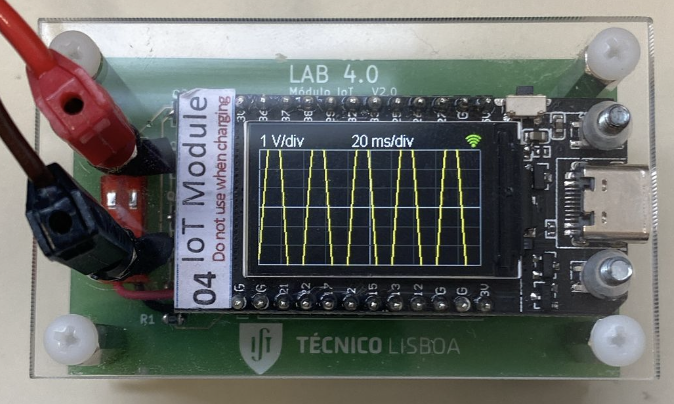
\includegraphics[width=1\linewidth]{Imagens/Testes no laboratório/Não calibrado/Vertical 1V.png}
        \captionsetup{justification=centering}
        \caption{1V/div e 20ms/div}
        \label{fig:1V/div e 20ms/div não calibrado}
    \end{subfigure}
    \begin{subfigure}{0.35\textwidth}
        \centering
        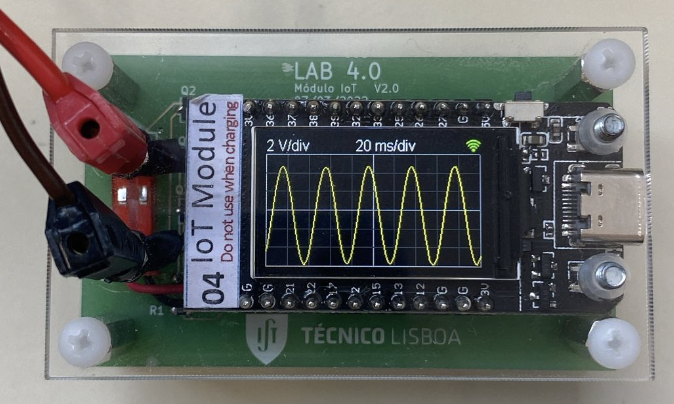
\includegraphics[width=1\linewidth]{Imagens/Testes no laboratório/Não calibrado/Vertical 2V.png}
        \captionsetup{justification=centering}
        \caption{2V/div e 20ms/div}
        \label{fig:2V/div e 20ms/div não calibrado}
    \end{subfigure}
    \begin{subfigure}{0.35\textwidth}
        \centering
        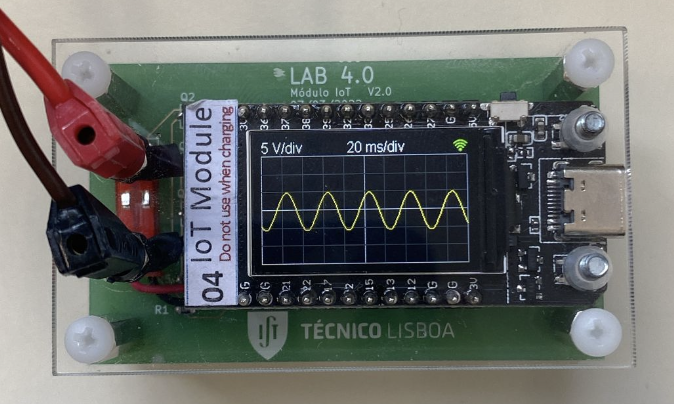
\includegraphics[width=1\linewidth]{Imagens/Testes no laboratório/Não calibrado/Vertical 5V.png}
        \captionsetup{justification=centering}
        \caption{5V/div e 20ms/div}
        \label{fig:5V/div e 20ms/div não calibrado}
    \end{subfigure}
    \begin{subfigure}{0.35\textwidth}
        \centering
        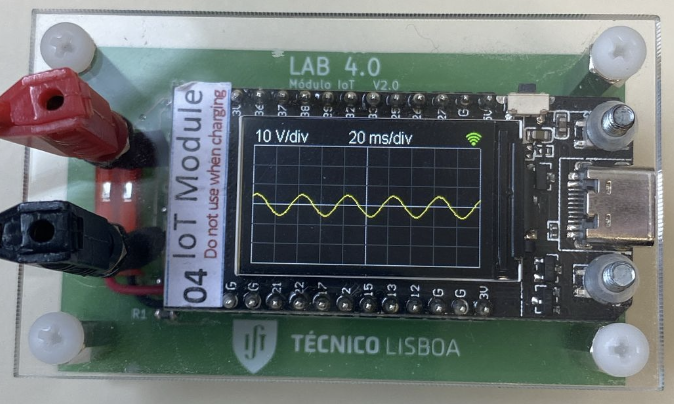
\includegraphics[width=1\linewidth]{Imagens/Testes no laboratório/Não calibrado/Vertical 10V.png}
        \captionsetup{justification=centering}
        \caption{10V/div e 20ms/div}
        \label{fig:10V/div e 20ms/div vertical não calibrado}
    \end{subfigure}
    \captionsetup{justification=centering}
    \caption{Variação da escala vertical (não calibrado)}
    \label{fig:Variação da escala vertical (não calibrado)}
\end{figure}

\begin{figure}[H]
    \centering
    \begin{subfigure}{0.35\textwidth}
        \centering
        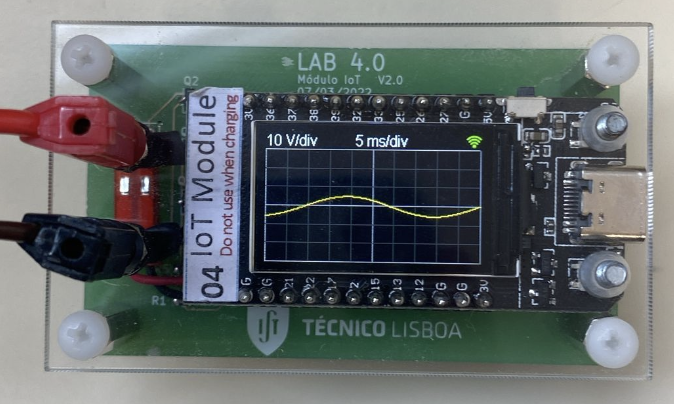
\includegraphics[width=1\linewidth]{Imagens/Testes no laboratório/Não calibrado/Horizontal 5ms.png}
        \captionsetup{justification=centering}
        \caption{10V/div e 5ms/div}
        \label{fig:10V/div e 5ms/div não calibrado}
    \end{subfigure}
    \begin{subfigure}{0.35\textwidth}
        \centering
        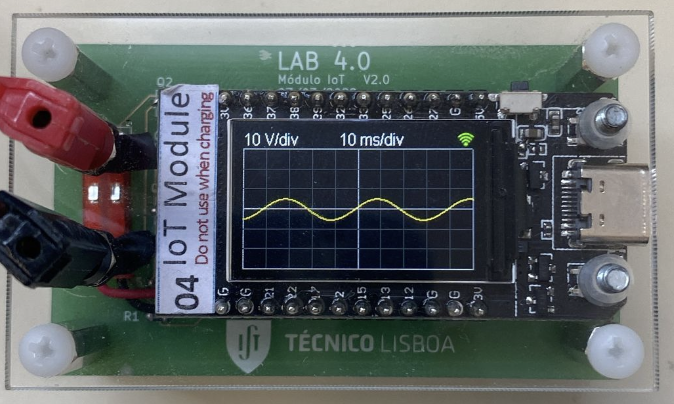
\includegraphics[width=1\linewidth]{Imagens/Testes no laboratório/Não calibrado/Horizontal 10ms.png}
        \captionsetup{justification=centering}
        \caption{10V/div e 10ms/div}
        \label{fig:10V/div e 10ms/div não calibrado}
    \end{subfigure}
    \begin{subfigure}{0.35\textwidth}
        \centering
        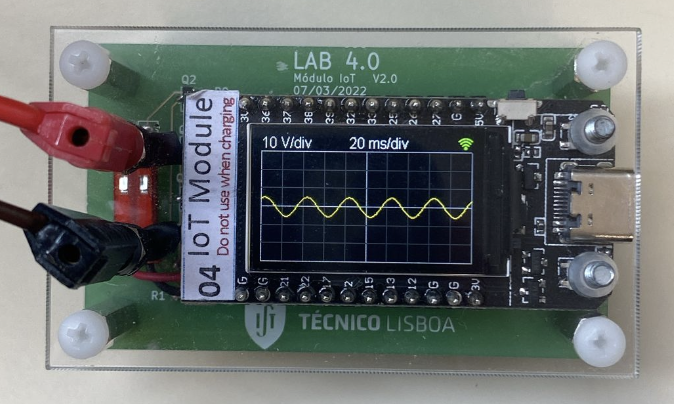
\includegraphics[width=1\linewidth]{Imagens/Testes no laboratório/Não calibrado/Horizontal 20ms.png}
        \captionsetup{justification=centering}
        \caption{10V/div e 20ms/div}
        \label{fig:10V/div e 20ms/div horizontal não calibrado}
    \end{subfigure}
    \begin{subfigure}{0.35\textwidth}
        \centering
        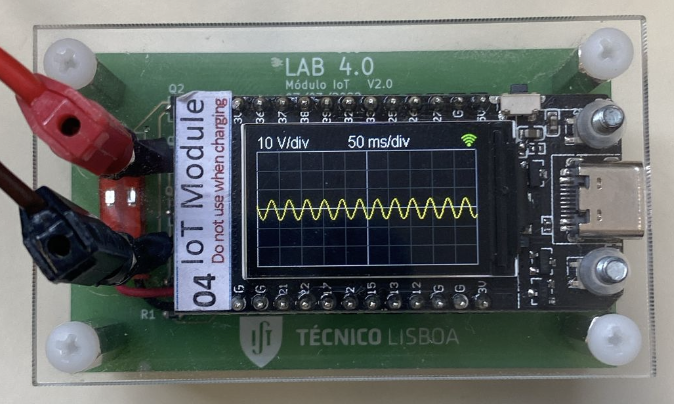
\includegraphics[width=1\linewidth]{Imagens/Testes no laboratório/Não calibrado/Horizontal 50ms.png}
        \captionsetup{justification=centering}
        \caption{10V/div e 50ms/div}
        \label{fig:10V/div e 50ms/div não calibrado}
    \end{subfigure}
    \captionsetup{justification=centering}
    \caption{Variação da escala horizontal (não calibrado)}
    \label{fig:Variação da escala horizontal (não calibrado)}
\end{figure}

\begin{figure}[H]
    \centering
    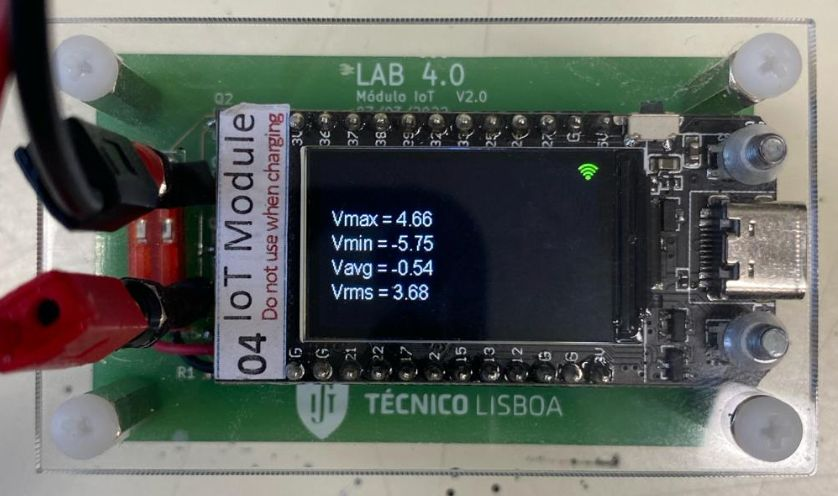
\includegraphics[width=0.35\textwidth]{Imagens/Testes no laboratório/Não calibrado/Botão 13.jpeg}
    \captionsetup{justification=centering}
    \caption{Funcionamento do duplo clique do botão 1 (não calibrado)}
    \label{fig:Funcionamento do duplo clique do botão 1 (não calibrado)}
\end{figure}

\vspace{-0.25cm}

\begin{figure}[H]
    \centering
    \begin{subfigure}{0.35\textwidth}
        \centering
        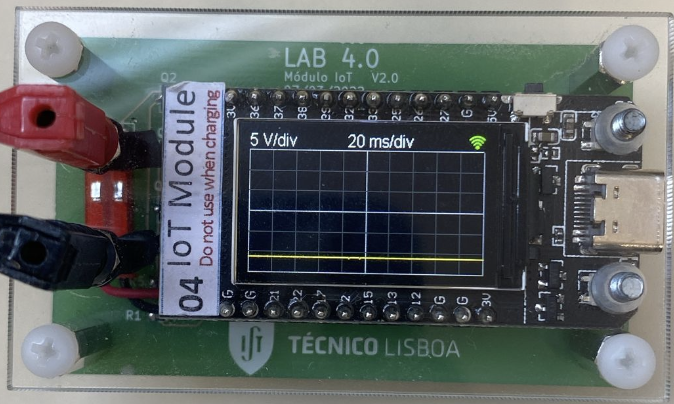
\includegraphics[width=1\linewidth]{Imagens/Testes no laboratório/Não calibrado/DC -10V.png}
        \captionsetup{justification=centering}
        \caption{DC -10V}
        \label{fig:DC -10V não calibrado}
    \end{subfigure}
    \begin{subfigure}{0.35\textwidth}
        \centering
        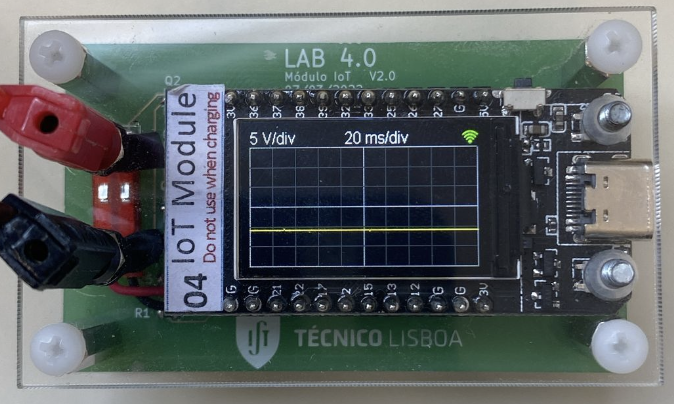
\includegraphics[width=1\linewidth]{Imagens/Testes no laboratório/Não calibrado/DC -5V.png}
        \captionsetup{justification=centering}
        \caption{DC -5V}
        \label{fig:DC -5V não calibrado}
    \end{subfigure}
    \begin{subfigure}{0.35\textwidth}
        \centering
        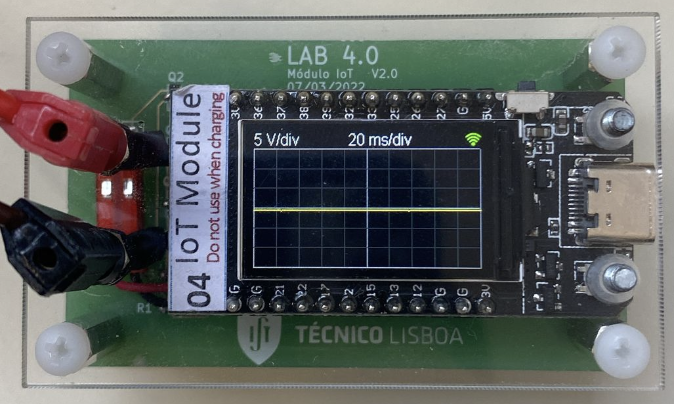
\includegraphics[width=1\linewidth]{Imagens/Testes no laboratório/Não calibrado/DC 0V.png}
        \captionsetup{justification=centering}
        \caption{DC 0V}
        \label{fig:DC 0V não calibrado}
    \end{subfigure}
    \begin{subfigure}{0.35\textwidth}
        \centering
        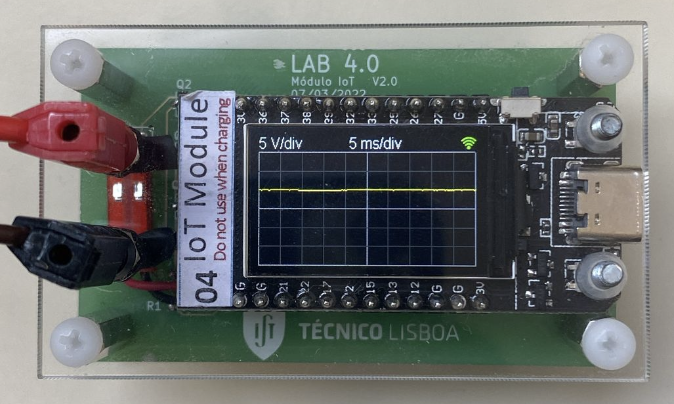
\includegraphics[width=1\linewidth]{Imagens/Testes no laboratório/Não calibrado/DC 5V.png}
        \captionsetup{justification=centering}
        \caption{DC 5V}
        \label{fig:DC 5V não calibrado}
    \end{subfigure}
\end{figure}

\begin{figure}[H]\ContinuedFloat
    \centering
    \begin{subfigure}{0.35\textwidth}
        \centering
        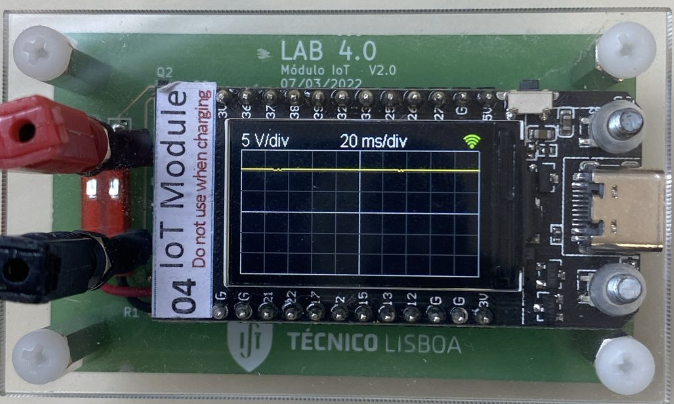
\includegraphics[width=1\linewidth]{Imagens/Testes no laboratório/Não calibrado/DC 10V.png}
        \captionsetup{justification=centering}
        \caption{DC 10V}
        \label{fig:DC 10V não calibrado}
    \end{subfigure}
    \captionsetup{justification=centering}
    \caption{Variação de uma tensão DC (não calibrado)}
    \label{fig:Variação de uma tensão DC (não calibrado)}
\end{figure}

\begin{figure}[H]
    \centering
    \begin{subfigure}{0.35\textwidth}
        \centering
        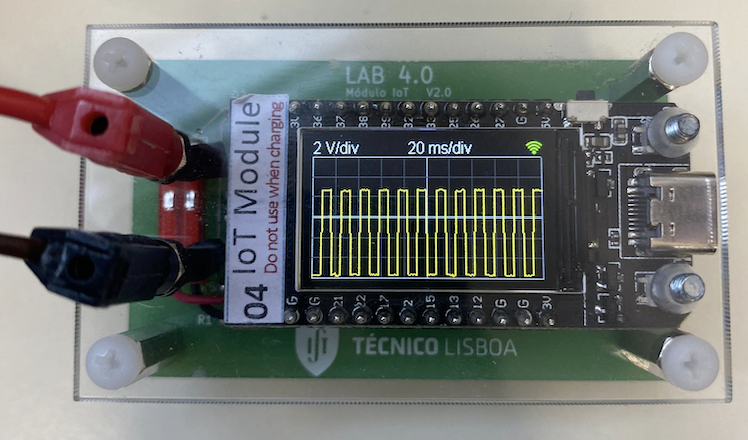
\includegraphics[width=1\linewidth]{Imagens/Testes no laboratório/Não calibrado/Onda quadrada do enunciado.png}
        \captionsetup{justification=centering}
        \caption{Onda quadrada}
        \label{fig:Onda quadrada não calibrado}
    \end{subfigure}
    \begin{subfigure}{0.35\textwidth}
        \centering
        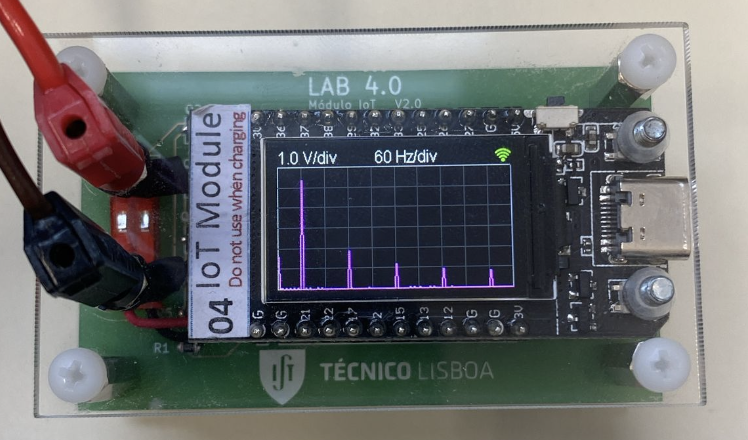
\includegraphics[width=1\linewidth]{Imagens/Testes no laboratório/Não calibrado/Onda quadrada do enunciado espetro.png}
        \captionsetup{justification=centering}
        \caption{Espetro da onda quadrada}
        \label{fig:Espetro da onda quadrada não calibrado}
    \end{subfigure}
    \captionsetup{justification=centering}
    \caption{Onda quadrada do enunciado e o seu espetro (não calibrado)}
    \label{fig:Onda quadrada do enunciado e o seu espetro (não calibrado)}
\end{figure}

Como era de esperar, verifica-se a necessidade de calibrar o sistema por mera observação das imagens acima no que toca à incorreta representação dos sinais e, nomeadamente, o erro associado ao conjunto de medidas evidenciado na \autoref{fig:Funcionamento do duplo clique do botão 1 (não calibrado)} (facilmente observável pelas tensões máxima e mínima apresentadas).